\section{Practical Session 2: Three-Phase Circuits and Power Transfer}

\subsection{Exercises}
\begin{enumerate}
    \item \textbf{Balanced Three-Phase Voltage Source Phasors and Waveforms}\footnote{Exercises 2.11, 2.12, 2.16, 2.17, 2.18, 2.19 and 2.20 from Ned Mohan's book \textit{"Electric power systems, a first course"}.}
    
    A positive sequence ($a$-$b$-$c$), balanced, wye-connected voltage source has the phase-$a$ RMS phasor voltage given by:
    \[
    \bar{V}_a = \sqrt{2} \times 100 e^{j 30^\circ}\ \text{V}.
    \]
    Obtain the time-domain voltages $v_a(t)$, $v_b(t)$, $v_c(t)$ and $v_{ab}(t)$, and show all of these as phasors in a phasor diagram.

    \item \textbf{Balanced Three-Phase Inductive Load}
    
    A balanced three-phase inductive load is supplied in steady state by a balanced, wye-connected, three-phase voltage source with a phase voltage of $120\ \text{V}$ RMS. The load draws a total active power of $10\ \text{kW}$ at a power factor of $0.9$ (inductive).
    \begin{enumerate}
        \item Calculate the RMS value of the phase currents.
        \item Calculate the magnitude and phase of the per-phase load impedance, assuming a wye-connected load.
        \item Draw a phasor diagram showing all three phase voltages and currents.
    \end{enumerate}

    \item \textbf{Power Transfer Between Two AC Systems}
    
    In the per-phase circuit of Figure~\ref{fig:tp2_powertransfer}, the active power transfer per phase is $P = 1\ \text{kW}$ from side $S$ (sending) to side $R$ (receiving). The parameters are:
    \[
    V_S = 100\ \text{V},\quad \bar{V}_R = 95\angle 0^\circ\ \text{V},\quad X = 1.5\ \Omega.
    \]
    Calculate the line current $\bar{I}$, the phase angle $\theta_S$ of $\bar{V}_S$, and the per-phase reactive power $Q_R$ supplied to the receiving end.

    \begin{figure}[htbp]
        \centering
        \begin{circuitikz}[american, scale=1.1]
            \draw (0,0) to[sV, v_>=$\bar{V}_S$] (0,2.5)
                  to[short, i=$\bar{I}$] (1.5,2.5)
                  to[L, l=$jX$] (3.5,2.5)
                  -- (5,2.5)
                  to[sV, v<=$\bar{V}_R$] (5,0)
                  -- (0,0);
            \node[above=0.2cm] at (0,2.5) {$S_S = \bar{V}_S \bar{I}^*$};
            \node[above=0.2cm] at (5,2.5) {$S_R = \bar{V}_R \bar{I}^*$};
        \end{circuitikz}
        \caption{Per-phase model of power transfer between two AC systems.}
        \label{fig:tp2_powertransfer}
    \end{figure}

    \item \textbf{Voltage Profile of a Radial Transmission System}
    
    In a radial system represented by the circuit of Figure~\ref{fig:tp2_powertransfer} where the receiving end is a passive load, the series reactance is $X = 1.5\ \Omega$. Consider the sending-end voltage to be held constant at $\bar{V}_S = 100\angle 0^\circ\ \text{V}$.
    \begin{enumerate}
        \item Derive a formula for $Q_R$, the reactive power consumed by the load, in terms of $P_R$ and the power factor $\cos\phi$.
        \item Derive a second-order polynomial equation for $V_R^2$ that depends on $X$, $V_S$, $P_R$, and $Q_R$.
        \item Calculate and discuss the ratio $V_S/V_R$ and the power angle $\delta$ when the active load $P_R$ varies from $0$ to $1\ \text{kW}$ for three power factors:
        \begin{itemize}
            \item Unity ($\cos\phi = 1.0$)
            \item Inductive ($\cos\phi = 0.9$ lagging)
            \item Capacitive ($\cos\phi = 0.9$ leading)
        \end{itemize}
    \end{enumerate}

    \item \textbf{Per-Unit Analysis of a Three-Phase System}
    
    In the balanced three-phase circuit of Figure~\ref{fig:tp2_wye}, the load impedance magnitude is $|Z_L| = 10\ \Omega$ per phase, and the per-phase power factor is $0.8$ (lagging).
    Calculate the base values, the per-unit values of the load impedance $Z_{L,pu}$, and the load real and reactive powers $P_{1\phi,pu}$ and $Q_{1\phi,pu}$ for each of the following base specifications:
    \begin{enumerate}
        \item Line-to-line voltage base $U^B = 208\ \text{V}$, three-phase power base $S_{3\phi}^B = 3.6\ \text{kVA}$.
        \item Line-to-line voltage base $U^B = 240\ \text{V}$, three-phase power base $S_{3\phi}^B = 5.4\ \text{kVA}$.
        \item Line-to-line voltage base $U^B = 240\ \text{V}$, three-phase power base $S_{3\phi}^B = 3.6\ \text{kVA}$.
    \end{enumerate}

    \begin{figure}[htbp]
        \centering
        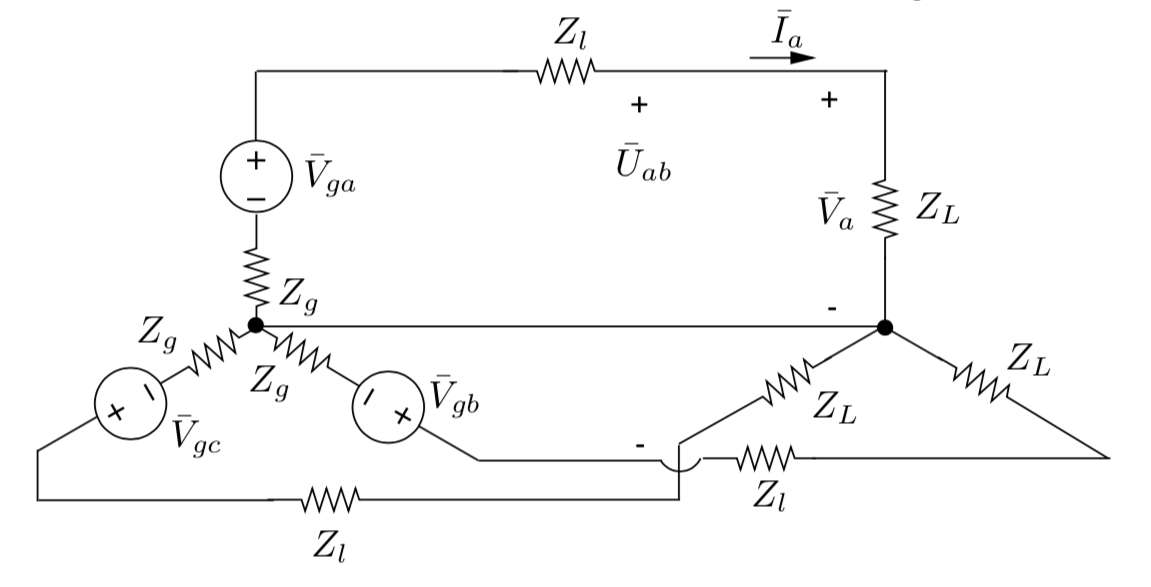
\includegraphics[width=0.72\linewidth]{../Lectures/ThreePhaseAndPu/images/three-phase-system.png}
        \caption{Balanced wye-connected three-phase source and load system.}
        \label{fig:tp2_wye}
    \end{figure}
\end{enumerate}

\newpage
\subsection{Solutions}

\subsubsection*{Solution to Exercise 1: Three-Phase Source Phasors and Waveforms}
\paragraph{Data:}
Positive sequence ($a$-$b$-$c$) balanced source with:
\[
\bar{V}_a = \sqrt{2} \times 100 e^{j 30^\circ}\ \text{V} = 141.42\ \text{V} \angle 30^\circ = 122.47 + j70.71\ \text{V}
\]
Since the phasor is given in RMS, the amplitude of the time-domain sinusoidal wave is $\sqrt{2} \times |\bar{V}_a| = \sqrt{2} \times 141.42 = 200\ \text{V}$.

\paragraph{Time-Domain Voltages:}
\begin{align}
    \boxed{v_a(t) = 200 \cos(\omega t + 30^\circ)\ \text{V}}
\end{align}
In a balanced positive-sequence system, phase $b$ lags phase $a$ by $120^\circ$, and phase $c$ leads phase $a$ by $120^\circ$ (or lags by $240^\circ$):
\begin{align}
    \bar{V}_b &= \bar{V}_a e^{-j 120^\circ} = \sqrt{2} \times 100 e^{j (30^\circ - 120^\circ)} \nonumber\\
              &= \sqrt{2} \times 100 e^{-j 90^\circ} = -j 141.42\ \text{V} \\
    \boxed{v_b(t) = 200 \cos(\omega t - 90^\circ)\ \text{V}}
\end{align}
\begin{align}
    \bar{V}_c &= \bar{V}_a e^{+j 120^\circ} = \sqrt{2} \times 100 e^{j (30^\circ + 120^\circ)} \nonumber\\
              &= \sqrt{2} \times 100 e^{j 150^\circ} = -122.47 + j 70.71\ \text{V} \\
    \boxed{v_c(t) = 200 \cos(\omega t + 150^\circ)\ \text{V}}
\end{align}

\paragraph{Line-to-Line Voltage $\bar{V}_{ab}$:}
\begin{align}
    \bar{V}_{ab} &= \bar{V}_a - \bar{V}_b = \sqrt{2} \times 100 \left( e^{j 30^\circ} - e^{-j 90^\circ} \right) \nonumber\\
                 &= (122.47 + j 70.71) - (-j 141.42) = 122.47 + j 212.13\ \text{V} \nonumber\\
                 &= 244.95\ \text{V} \angle 60^\circ = \sqrt{3} \bar{V}_a e^{j 30^\circ}
\end{align}
The peak amplitude is $200 \sqrt{3} = 346.41\ \text{V}$:
\begin{equation}
    \boxed{v_{ab}(t) = 200\sqrt{3} \cos(\omega t + 60^\circ)\ \text{V} = 346.41 \cos(\omega t + 60^\circ)\ \text{V}}
\end{equation}

\begin{figure}[htbp]
    \centering
    \begin{tikzpicture}[scale=1.5, >=Stealth]
        % Axes
        \draw[thin, gray!40] (-2.2,-2.2) grid (2.2,2.2);
        \draw[->, thick] (-2.2,0) -- (2.2,0) node[right] {$\text{Re}$};
        \draw[->, thick] (0,-2.2) -- (0,2.2) node[above] {$\text{Im}$};
        \draw[dashed, gray] (0,0) circle (1.414);

        % Phasors
        \draw[->, very thick, blue] (0,0) -- (30:1.414) node[above right] {$\bar{V}_a = 141.4\angle 30^\circ$};
        \draw[->, very thick, blue] (0,0) -- (-90:1.414) node[below right] {$\bar{V}_b = 141.4\angle -90^\circ$};
        \draw[->, very thick, blue] (0,0) -- (150:1.414) node[above left] {$\bar{V}_c = 141.4\angle 150^\circ$};
        \draw[->, dashed, thick, gray] (0,0) -- (90:1.414) node[above right] {$-\bar{V}_b$};

        % Line-to-line Vab
        \draw[->, very thick, red] (0,0) -- (60:2.45) node[above right] {$\bar{V}_{ab} = \bar{V}_a - \bar{V}_b = 244.95\angle 60^\circ$};
        \draw[dotted, thick, red] (30:1.414) -- (60:2.45);
        \draw[dotted, thick, red] (90:1.414) -- (60:2.45);
    \end{tikzpicture}
    \caption{Phasor diagram of balanced phase voltages and line-to-line voltage $\bar{V}_{ab}$.}
    \label{fig:tp2_phasor1}
\end{figure}

\subsubsection*{Solution to Exercise 2: Balanced Three-Phase Inductive Load}
\paragraph{Data:}
\begin{itemize}
    \item Phase voltage: $V_{1\phi} = 120\ \text{V}$ RMS
    \item Total 3-phase active power: $P_{3\phi} = 10\ \text{kW} = 10^4\ \text{W}$
    \item Power factor: $\cos\phi = 0.9$ (inductive/lagging) $\implies \phi = +\arccos(0.9) = +25.842^\circ$
\end{itemize}

\paragraph{1. Phase Current RMS Value:}
The per-phase active power is:
\[
P_{1\phi} = \frac{P_{3\phi}}{3} = \frac{10^4}{3} = 3333.33\ \text{W}
\]
Using $P_{1\phi} = V_{1\phi} I_{\text{RMS}} \cos\phi$:
\begin{equation}
    \boxed{I_{\text{RMS}} = \frac{P_{1\phi}}{V_{1\phi} \cos\phi} = \frac{3333.33}{120 \times 0.9} = 30.86\ \text{A}}
\end{equation}

\paragraph{2. Load Impedance $Z_{1\phi}$:}
For a wye connection, the voltage across each phase impedance is the phase voltage $V_{1\phi} = 120\ \text{V}$:
\begin{equation}
    |Z_{1\phi}| = \frac{V_{1\phi}}{I_{\text{RMS}}} = \frac{120}{30.864} = 3.888\ \Omega
\end{equation}
Since the load is inductive, current lags voltage by $\phi = 25.84^\circ$, meaning the impedance angle is positive:
\begin{equation}
    \boxed{Z_{1\phi} = 3.888\ \Omega \angle +25.84^\circ = (3.50 + j1.70)\ \Omega}
\end{equation}

\paragraph{3. Phasor Diagram:}
Taking $\bar{V}_a = 120\angle 0^\circ\ \text{V}$ as reference:
\begin{itemize}
    \item Voltages: $\bar{V}_a = 120\angle 0^\circ\ \text{V}$, $\bar{V}_b = 120\angle -120^\circ\ \text{V}$, $\bar{V}_c = 120\angle +120^\circ\ \text{V}$
    \item Currents: $\bar{I}_a = 30.86\ \text{A} \angle -25.84^\circ$, $\bar{I}_b = 30.86\ \text{A} \angle -145.84^\circ$, $\bar{I}_c = 30.86\ \text{A} \angle +94.16^\circ$
\end{itemize}

\begin{figure}[htbp]
    \centering
    \begin{tikzpicture}[scale=1.4, >=Stealth]
        \draw[thin, gray!40] (-2.2,-2.2) grid (2.2,2.2);
        \draw[->, thick] (-2.2,0) -- (2.2,0) node[right] {$\text{Re}$};
        \draw[->, thick] (0,-2.2) -- (0,2.2) node[above] {$\text{Im}$};

        % Voltages (scaled to length 1.8)
        \draw[->, very thick, blue] (0,0) -- (0:1.8) node[right] {$\bar{V}_a$};
        \draw[->, very thick, blue] (0,0) -- (-120:1.8) node[below left] {$\bar{V}_b$};
        \draw[->, very thick, blue] (0,0) -- (120:1.8) node[above left] {$\bar{V}_c$};

        % Currents (scaled to length 1.2)
        \draw[->, very thick, red] (0,0) -- (-25.84:1.2) node[right] {$\bar{I}_a$};
        \draw[->, very thick, red] (0,0) -- (-145.84:1.2) node[below left] {$\bar{I}_b$};
        \draw[->, very thick, red] (0,0) -- (94.16:1.2) node[above] {$\bar{I}_c$};

        % Angle arc
        \draw[->, thick, domain=0:-25.84] plot ({0.7*cos(\x)}, {0.7*sin(\x)});
        \node[right] at (-12:0.7) {$\phi = 25.8^\circ$};
    \end{tikzpicture}
    \caption{Phasor diagram of voltages and lagging currents for the balanced inductive load.}
    \label{fig:tp2_phasor2}
\end{figure}

\subsubsection*{Solution to Exercise 3: Power Transfer Between Two AC Systems}
\paragraph{Data:}
\begin{itemize}
    \item Transferred active power: $P = 1\ \text{kW} = 1000\ \text{W}$
    \item Sending-end voltage: $V_S = 100\ \text{V}$ (angle $\theta_S$ to be determined)
    \item Receiving-end voltage: $\bar{V}_R = 95\ \text{V}\angle 0^\circ \implies V_R = 95\ \text{V}$, $\theta_R = 0^\circ$
    \item Line reactance: $X = 1.5\ \Omega$ (lossless line, $R = 0$)
\end{itemize}

\paragraph{Derivation of Power Transfer Formulas:}
The line current directed from $S$ to $R$ is:
\begin{equation}
    \bar{I} = \frac{\bar{V}_S - \bar{V}_R}{jX}
\end{equation}
The complex power injected by the sending-end source $S$ is:
\begin{align}
    S_S &= \bar{V}_S \bar{I}^* = \bar{V}_S \left(\frac{\bar{V}_S - \bar{V}_R}{jX}\right)^* = \frac{V_S^2 - \bar{V}_S \bar{V}_R^*}{-jX} = j \frac{V_S^2 - V_S V_R e^{j(\theta_S - \theta_R)}}{X} \nonumber\\
        &= \frac{V_S V_R \sin(\theta_S - \theta_R)}{X} + j \frac{V_S^2 - V_S V_R \cos(\theta_S - \theta_R)}{X}
\end{align}
Hence:
\begin{align}
    P_S &= \frac{V_S V_R \sin(\theta_S - \theta_R)}{X} \label{eq:PS_formula}\\
    Q_S &= \frac{V_S^2 - V_S V_R \cos(\theta_S - \theta_R)}{X} \label{eq:QS_formula}
\end{align}

\paragraph{Phase Angle $\theta_S$:}
Since the line is lossless ($R = 0$), $P_S = P_R = 1000\ \text{W}$. With $\theta_R = 0^\circ$:
\begin{equation}
    \sin\theta_S = \frac{X P_S}{V_S V_R} = \frac{1.5 \times 1000}{100 \times 95} = \frac{1500}{9500} = 0.15789
\end{equation}
\begin{equation}
    \boxed{\theta_S = \arcsin(0.15789) = 9.085^\circ\quad (0.1585\ \text{rad})}
\end{equation}

\paragraph{Line Current $\bar{I}$:}
\begin{align}
    \bar{I} &= \frac{100\angle 9.085^\circ - 95\angle 0^\circ}{j 1.5} = \frac{(98.743 + j15.789) - 95}{j 1.5} \nonumber\\
            &= \frac{3.743 + j15.789}{j 1.5} = \frac{15.789 - j3.743}{1.5} = 10.526 - j2.495\ \text{A} \nonumber\\
            &= \boxed{10.818\ \text{A} \angle -13.35^\circ}
\end{align}

\paragraph{Per-Phase Reactive Power $Q_R$ Supplied to the Receiving End:}
The power received at bus $R$ is:
\begin{align}
    S_R &= \bar{V}_R \bar{I}^* = (95\angle 0^\circ)(10.526 + j2.495) \nonumber\\
        &= 999.97 + j237.06\ \text{VA} \approx 1000\ \text{W} + j 237.22\ \text{var}
\end{align}
Alternatively, using the analytical receiving-end formula:
\begin{align}
    Q_R &= \text{Im}\{\bar{V}_R \bar{I}^*\} = \frac{V_S V_R \cos(\theta_R - \theta_S) - V_R^2}{X} \nonumber\\
        &= \frac{100 \times 95 \times \cos(-9.085^\circ) - 95^2}{1.5} \nonumber\\
        &= \frac{9500 \times 0.9874 - 9025}{1.5} = \frac{9380.57 - 9025}{1.5} = \boxed{237.05\ \text{var} \approx 237.22\ \text{var}}
\end{align}
\textit{Note on sign convention:} As annotated in the handwritten notes, $Q_R > 0$ indicates that the line supplies $237.22\ \text{var}$ of reactive power into the receiving-end source/bus.

\subsubsection*{Solution to Exercise 4: Voltage Profile of a Radial Transmission System}
\paragraph{(a) Load Reactive Power $Q_R$:}
Let the load complex power be $S_R = P_R + j Q_R$. By definition of the load power factor:
\begin{equation}
    \cos\phi = \frac{P_R}{|S_R|} = \frac{P_R}{\sqrt{P_R^2 + Q_R^2}} \iff Q_R = \pm P_R \sqrt{\frac{1}{\cos^2\phi} - 1}
\end{equation}
\begin{itemize}
    \item \textbf{Unity power factor ($\cos\phi = 1$):} $Q_R = 0$.
    \item \textbf{Lagging power factor ($\cos\phi = 0.9$):} $Q_R = + P_R \sqrt{\frac{1}{0.9^2} - 1} = +0.4843 P_R > 0$ (inductive load consumes reactive power).
    \item \textbf{Leading power factor ($\cos\phi = 0.9$):} $Q_R = - P_R \sqrt{\frac{1}{0.9^2} - 1} = -0.4843 P_R < 0$ (capacitive load generates reactive power).
\end{itemize}

\paragraph{(b) Second-Order Equation for $V_R^2$:}
Let $\delta = \theta_R - \theta_S$ be the transmission angle. The power flow equations at the receiving end are:
\begin{align}
    P_R &= \frac{V_S V_R \sin\delta}{X} \implies V_R \sin\delta = \frac{P_R X}{V_S} \label{eq:radial_sin}\\
    Q_R &= \frac{V_S V_R \cos\delta - V_R^2}{X} \implies V_R \cos\delta = \frac{X Q_R + V_R^2}{V_S} \label{eq:radial_cos}
\end{align}
Squaring and summing equations~\eqref{eq:radial_sin} and~\eqref{eq:radial_cos}:
\begin{equation}
    V_R^2 (\sin^2\delta + \cos^2\delta) = V_R^2 = \left(\frac{P_R X}{V_S}\right)^2 + \left(\frac{X Q_R + V_R^2}{V_S}\right)^2
\end{equation}
Multiplying both sides by $V_S^2$:
\begin{equation}
    V_S^2 V_R^2 = P_R^2 X^2 + X^2 Q_R^2 + 2 X Q_R V_R^2 + V_R^4
\end{equation}
Rearranging terms into standard polynomial form in $y = V_R^2$:
\begin{equation}
    \boxed{y^2 + (2X Q_R - V_S^2) y + X^2 (P_R^2 + Q_R^2) = 0\quad \text{with}\quad y = V_R^2}
\end{equation}

\paragraph{(c) Ratio $V_S/V_R$ and Power Angle $\delta$:}
Solving the quadratic equation for $y = V_R^2$:
\begin{equation}
    V_R^2 = \frac{-(2X Q_R - V_S^2) + \sqrt{(2X Q_R - V_S^2)^2 - 4 X^2(P_R^2 + Q_R^2)}}{2}
\end{equation}
(choosing the positive square root corresponding to normal, stable operating voltage).
Once $V_R$ is obtained, the power angle $\delta$ is:
\begin{equation}
    \delta = \arcsin\left(\frac{P_R X}{V_S V_R}\right)
\end{equation}

\paragraph{Physical Interpretation:}
\begin{itemize}
    \item \textbf{Lagging power factor (inductive):} As $P_R$ increases, the line reactive drop adds to the load reactive demand, causing a severe drop in receiving voltage $V_R$, so $V_S/V_R > 1$ increases rapidly.
    \item \textbf{Unity power factor:} $V_R$ exhibits a moderate voltage drop due to the line series reactance.
    \item \textbf{Leading power factor (capacitive):} The capacitive reactive power supports the voltage (Ferranti-like compensation effect), keeping $V_R$ elevated ($V_S/V_R \approx 1$ or even $< 1$ for light loads).
\end{itemize}

\subsubsection*{Solution to Exercise 5: Per-Unit Analysis of a Three-Phase System}
\paragraph{Data:}
\begin{itemize}
    \item Impedance magnitude: $|Z_L| = 10\ \Omega$
    \item Power factor: $\cos\phi = 0.8$ lagging $\implies \phi = \arccos(0.8) = +36.87^\circ$
    \item Load impedance: $Z_L = 10\ \Omega \angle 36.87^\circ = (8 + j6)\ \Omega$
\end{itemize}

\paragraph{Per-Unit Formulas:}
\begin{itemize}
    \item Phase voltage base: $V^B = \frac{U^B}{\sqrt{3}}$
    \item Single-phase power base: $S_{1\phi}^B = \frac{S_{3\phi}^B}{3}$
    \item Current base: $I^B = \frac{S_{1\phi}^B}{V^B} = \frac{S_{3\phi}^B}{\sqrt{3} U^B}$
    \item Base impedance: $Z^B = \frac{(V^B)^2}{S_{1\phi}^B} = \frac{(U^B)^2}{S_{3\phi}^B}$
\end{itemize}

\paragraph{Detailed Calculations for the Three Base Systems:}
\begin{table}[htbp]
    \centering
    \caption{Base quantities and per-unit values for Exercise 5.}
    \label{tab:tp2_pu}
    \renewcommand{\arraystretch}{1.3}
    \begin{tabular}{lccc}
        \toprule
        \textbf{Quantity} & \textbf{Case (a)} & \textbf{Case (b)} & \textbf{Case (c)} \\
        \midrule
        $U^B$ (line-to-line) & $208\ \text{V}$ & $240\ \text{V}$ & $240\ \text{V}$ \\
        $S_{3\phi}^B$ & $3.6\ \text{kVA}$ & $5.4\ \text{kVA}$ & $3.6\ \text{kVA}$ \\
        \midrule
        $V^B = U^B / \sqrt{3}$ & $120.09\ \text{V}$ & $138.56\ \text{V}$ & $138.56\ \text{V}$ \\
        $S_{1\phi}^B = S_{3\phi}^B / 3$ & $1.2\ \text{kVA}$ & $1.8\ \text{kVA}$ & $1.2\ \text{kVA}$ \\
        $I^B = S_{1\phi}^B / V^B$ & $10.0\ \text{A}$ & $13.0\ \text{A}$ & $8.66\ \text{A}$ \\
        $Z^B = (U^B)^2 / S_{3\phi}^B$ & $12.018\ \Omega$ & $10.667\ \Omega$ & $16.000\ \Omega$ \\
        \midrule
        $|Z_{L,pu}| = |Z_L| / Z^B$ & $0.832\ \text{pu}$ & $0.9375\ \text{pu}$ & $0.625\ \text{pu}$ \\
        $Z_{L,pu}$ & $\mathbf{0.832\angle 36.87^\circ\ \text{pu}}$ & $\mathbf{0.938\angle 36.87^\circ\ \text{pu}}$ & $\mathbf{0.625\angle 36.87^\circ\ \text{pu}}$ \\
        \midrule
        $|S_{1\phi}| = (V^B)^2 / |Z_L|$ & $1442.13\ \text{VA}$ & $1920.0\ \text{VA}$ & $1920.0\ \text{VA}$ \\
        $P_{1\phi} = |S_{1\phi}|\cos\phi$ & $1153.71\ \text{W}$ & $1536.0\ \text{W}$ & $1536.0\ \text{W}$ \\
        $Q_{1\phi} = |S_{1\phi}|\sin\phi$ & $865.28\ \text{var}$ & $1152.0\ \text{var}$ & $1152.0\ \text{var}$ \\
        \midrule
        $P_{pu} = P_{1\phi} / S_{1\phi}^B$ & $\mathbf{0.9614\ \text{pu}}$ & $\mathbf{0.8533\ \text{pu}}$ & $\mathbf{1.2800\ \text{pu}}$ \\
        $Q_{pu} = Q_{1\phi} / S_{1\phi}^B$ & $\mathbf{0.7213\ \text{pu}}$ & $\mathbf{0.6400\ \text{pu}}$ & $\mathbf{0.9600\ \text{pu}}$ \\
        \bottomrule
    \end{tabular}
\end{table}
Notice that in per-unit:
\[
S_{pu} = \frac{|V_{pu}|^2}{Z_{L,pu}^*} = \frac{1}{Z_{L,pu}^*} = \frac{1}{|Z_{L,pu}|} \angle 36.87^\circ
\]
For example, in case (a): $|S_{pu}| = 1 / 0.832 = 1.2018\ \text{pu}$, giving $P_{pu} = 1.2018 \times 0.8 = 0.9614\ \text{pu}$ and $Q_{pu} = 1.2018 \times 0.6 = 0.7211\ \text{pu}$, which matches perfectly.
